\section{Exact replenished-fleet constructions}\label{sec:exact}

Consider two mandatory depot-to-depot services.  Service A occupies hour
$[0,1]$ and service B occupies $[2,3]$; each consumes 15 kWh.  At most two
identical buses may be used.  Each used bus starts at its full 20 kWh
capacity and must return to 20 kWh by hour 4.  The early charging window is
$[1,2]$, with 10 kW per bus and in total.  The terminal window is $[3,4]$,
with 30 kW per bus and in total and enough connectors.  Charging is
continuous and lossless; reserve, travel cost, deadhead energy, auxiliary
load, switching time, and taper are zero.  No charging is available outside
these windows.  The terminal charge is physical replenishment, so its energy
and supply cost are included.

There are only two unlabeled service partitions.  If one bus covers A and B,
it reaches 5 kWh after A and needs at least 10 kWh before B.  The early
power limit fixes its early grid energy at $x=10$ kWh; it buys 20 kWh
terminally.  If two buses cover one service each, the A bus buys any
$x\in[0,10]$ kWh early and $15-x$ kWh terminally, while the B bus buys 15
kWh terminally.  Every used bus returns full.  Both structures therefore
buy exactly 30 kWh, and initial inventories cannot subsidize the horizon.

Let a used bus cost $f=7$ synthetic units and let grid supply cost be
\begin{equation}\label{eq:exact-supply}
 F(x,z)=4x+\frac{x^2+z^2}{10},\qquad x,z\geq0.
\end{equation}
The one-bus physical cost is $7+F(10,20)=97$.  The two-bus branch has cost
$14+F(x,30-x)$, minimized at $x=5$ with value 99.  Yet the complete-fleet
hull has a lower objective.

\begin{proposition}[Replenishment does not ensure price support]
\label{prop:exact-nominal}
For this physical model,
\begin{equation}\label{eq:exact-values}
 D=97,\qquad CH=\frac{7591}{80}=94.8875,\qquad
 \Delta=\frac{169}{80}=2.1125.
\end{equation}
The physical planner optimum has own-price regret 13.  At a common
hull-optimal price its fleet lost opportunity is zero and its supplier lost
opportunity is $169/80$.
\end{proposition}

The hull optimizer mixes the one-bus plan $(x,z)=(10,20)$ with weight
$27/40$ and the two-bus plan $(0,30)$ with weight $13/40$.  Its mean early
load is $27/4$ kWh.  Both components are physical; their mean load and mean
operating cost are a convexification, not a fractional bus schedule.  Running
the two plans on different days gives mean system cost 99.275, because
averaging physical supply costs differs from evaluating the convex supply
cost at their mean load.  The exact hull and price calculations are in
Appendix~\ref{app:theory-proofs}.

At the physical optimum, the own marginal price is $(6,4)$ synthetic
units/kWh.  The one-bus private objective is 147, while the two-bus plan
charging entirely terminally has private objective 134.  The resulting
13-unit regret is a fixed-price incentive to change the whole fleet.  The
hull price is $(5.35,4.65)$: the two plans supporting its mean tie at private
objective 153.5.  At that price, the physical one-bus optimum has no fleet
lost opportunity, but the supplier term is $169/80$.  These two diagnostics
use different prices and answer different questions.

Starting the undamped best-response iteration at the one-bus load gives the
exact two-cycle in Figure~\ref{fig:exact-cycle}. At $p=(6,4)$, one bus pays
147 and the two-bus fleet with load $(0,30)$ pays 134, so the response is two
buses. Updating the same supply gradient at that load gives $p=(4,6)$; now
the current two-bus plan pays 194, while the one-bus fleet with load
$(10,20)$ pays 167. Even the cheapest two-bus alternative at this price
costs 174. Both schedules fully replenish their buses. The iteration alternates
without damping or tie breaking. It illustrates this posted-price rule, not
a general claim about price-update algorithms.

\begin{figure}[t]
\centering
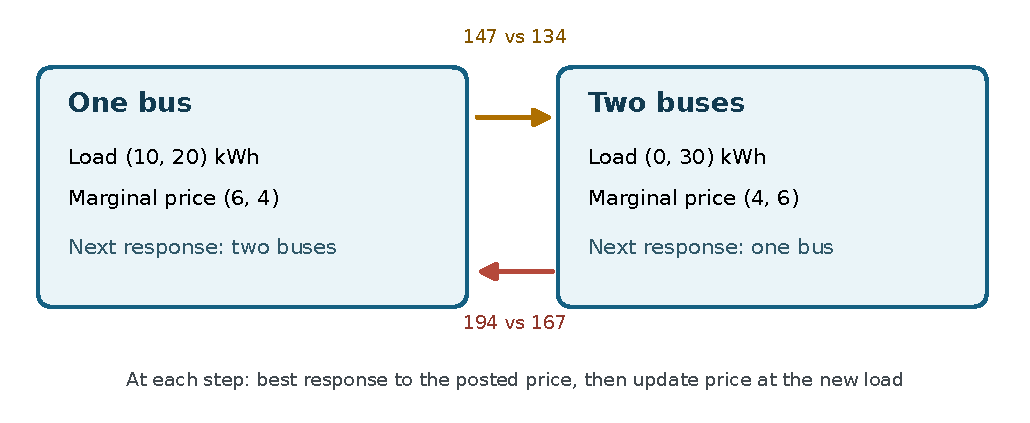
\includegraphics[width=.91\linewidth]{../figures/cyclic_price_update.pdf}
\caption{Exact undamped best-response cycle in the nominal two-service model.
Initialize at the one-bus physical optimum; each arrow holds the displayed
price fixed for the response, then updates to the marginal price of the new
load. Numbers on arrows compare the current fleet's bill with the responding
fleet's bill, in synthetic units.}
\label{fig:exact-cycle}
\end{figure}

\begin{figure}[t]
\centering
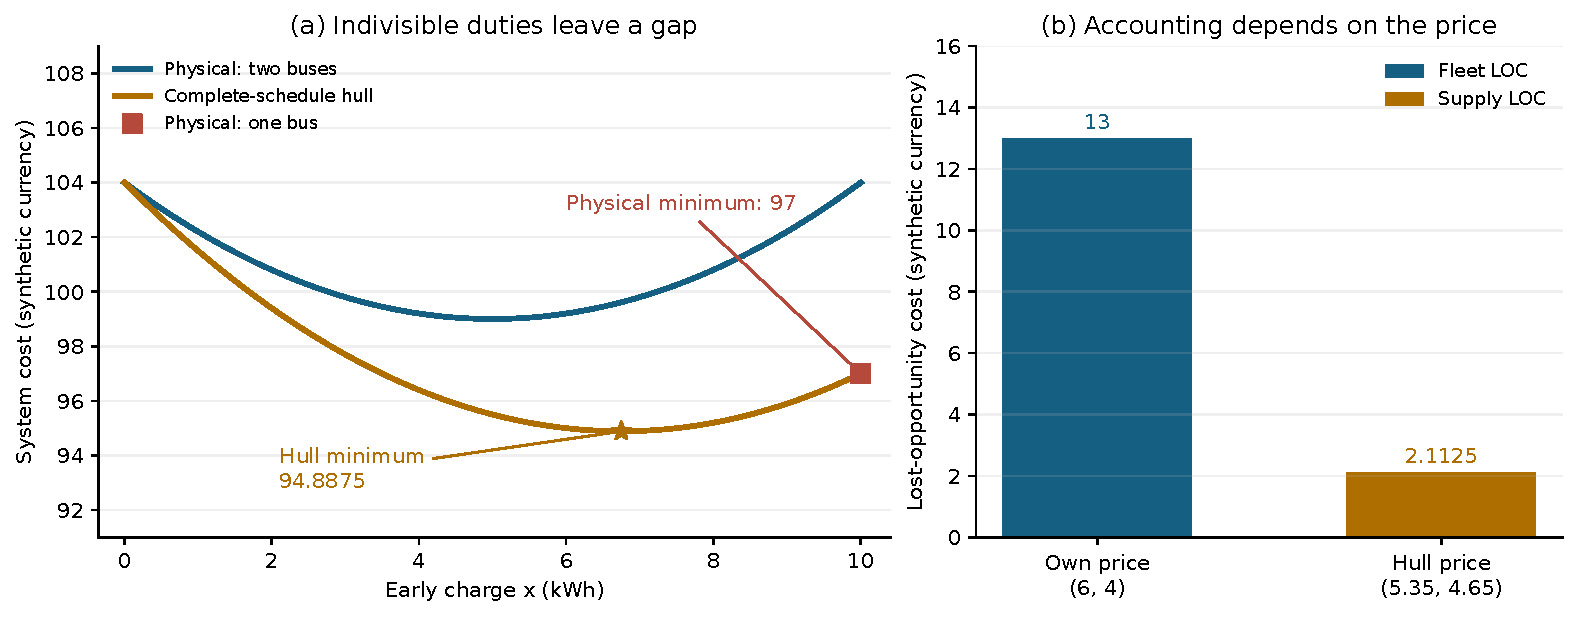
\includegraphics[width=.91\linewidth]{../figures/cyclic_gap_and_prices.pdf}
\caption{Exact physical branches, complete-fleet hull, and lost-opportunity
accounts in the synthetic two-service case.  Prices are synthetic units/kWh;
the hull mean is not an executable daily fleet.}
\label{fig:exact-gap}
\end{figure}

The binding 10 kW early limit is a fragile nominal parameter: at the same
20 kWh capacity, a positive reserve or charging loss can remove the
one-bus branch.  A nearby construction allows those constraints while
retaining a gap.  Keep two 15 kWh services, battery capacity 20, and
\eqref{eq:exact-supply}, but use reserve $r=1$ kWh, grid-to-battery
efficiency $\eta=19/20$, 12 kW individual and shared early power, and a
single 30 kW terminal connector.  The one-bus plan buys $220/19$ grid kWh
early and 20 terminally, with battery states
$20\to5\to16\to1\to20$.  Its early power has $8/19$ kWh of headroom.
The supporting two-bus plan buys $30/19$ early and 30 terminally; the two
terminal sessions take $9/19$ and $10/19$ hour and fit sequentially on the
single connector.  Every used bus again finishes full.

\begin{proposition}[A positive-gap neighborhood]\label{prop:exact-robust}
Under the modified parameters,
\begin{equation}\label{eq:exact-robust}
 D=\frac{38527}{361},\qquad
 CH=\frac{2987911}{28880},\qquad
 \Delta=\frac{94249}{28880}>0.
\end{equation}
With the 30 kW terminal connector fixed, strict feasible-headroom and
optimality inequalities preserve a positive gap in an open neighborhood
of the stated reserve, efficiency, and early power.
\end{proposition}

The interval and strict-inequality proof is in
Appendix~\ref{app:theory-proofs}.  The neighborhood is conditional on this
hardware model's zero switching time, constant efficiency, and lack of
taper.  For perspective on connector adequacy, if the original lossless
case has one terminal connector of power $K\leq30$ kW, it is infeasible for
$K<20$, has zero gap for $20\leq K\leq23.5$, and has a positive gap for
$23.5<K\leq30$.  Thus the presence of one connector alone says nothing
about price support.

\subsection{Replication and the participant scale}\label{sec:exact-replication}

Replicate A and B to $n$ simultaneous copies each.  Give the fleet $n$
early 10 kW connectors and $n$ terminal 30 kW connectors.  Battery and
service energy per bus stay fixed; supply cost scales with demand as
\begin{equation}\label{eq:exact-scaled-supply}
 F_n(E,L)=4E+\frac{E^2+L^2}{10n}.
\end{equation}
If $m$ buses each cover an A--B pair, $n-m$ A-only and $n-m$ B-only buses
complete the services.  There are $2n-m$ used buses, and physical early
energy ranges over $[10m,10n]$.  Terminal sessions have an explicit
connector-feasible assignment: paired buses take $m$ connectors, while
each A-only/B-only pair can share one of the other $n-m$ terminal
connectors sequentially.  All buses return full.

\begin{proposition}[A vanishing gap with aggregate regret]
\label{prop:exact-replication}
The complete projected hull has lower operating-cost boundary
$14n-0.7E$ and optimum $CH_n=7591n/80$.  Every physical optimum takes an
integer $m$ nearest to $27n/40$; both neighboring integers are retained at
a tie.  With $\delta=m-27n/40$,
\begin{equation}\label{eq:exact-replication-gap}
 \Delta_n=\frac{20\delta^2}{n}\leq\frac5n.
\end{equation}
Along $n=40k+1$, the whole-operator own-price regret is
\begin{equation}\label{eq:exact-replication-regret}
 r_n=\frac{351}{40}+\frac{169}{40n}\longrightarrow\frac{351}{40},
 \qquad
 \Delta_n=\frac{169}{80n}\longrightarrow0.
\end{equation}
For multiples of 40, both quantities are exactly zero.
\end{proposition}

The planning gap and the whole-operator incentive decouple:
$\Delta_n=O(1/n)$, yet $r_n$ stays bounded away from zero along
$n=40k+1$. Both are bounded independently of $n$ in this family, but only
the gap vanishes along that subsequence. Regret per bus and regret as a
fraction of physical cost also vanish. Shapley--Folkman theory explains why
sums of small nonconvex participants can become approximately convex
\citep{starr1969,hreinsson2021}; the exact rates here show why a small
planning gap alone does not control the absolute incentive of the operator
that owns the entire sum.

Now divide ownership among $n$ operators, each with one A/B service pair
and reserved early and terminal connectors. Each can choose the one-bus
plan or any two-bus plan with $x\in[0,10]$, and these deviations remain
compatible with the others' connector rights. At the physical optimum's
marginal price, each participant's regret is at most $20/n$. Their regrets
sum to the whole-fleet regret in this symmetric construction. Along
$n=40k+1$, each dissatisfied one-bus owner can gain only $13/n$, even
though their total gain tends to $351/40$. At $n=20$, the two tied planner
optima have whole-fleet regrets 7 and 14.

With separate ownership, each participant becomes negligible relative to
the growing market and its incentive vanishes. This is a small-participant
analogue of the divisible traffic flows coordinated by
\citet{alizadeh2016coupled}. With common ownership, the operator can instead
change the entire fleet at once. These two ends of the participant scale
connect the aggregation argument to the coordination model in
Section~\ref{sec:generation}; they do not identify the reserved-connector
model with Alizadeh et al.'s transportation network.

\begin{figure}[t]
\centering
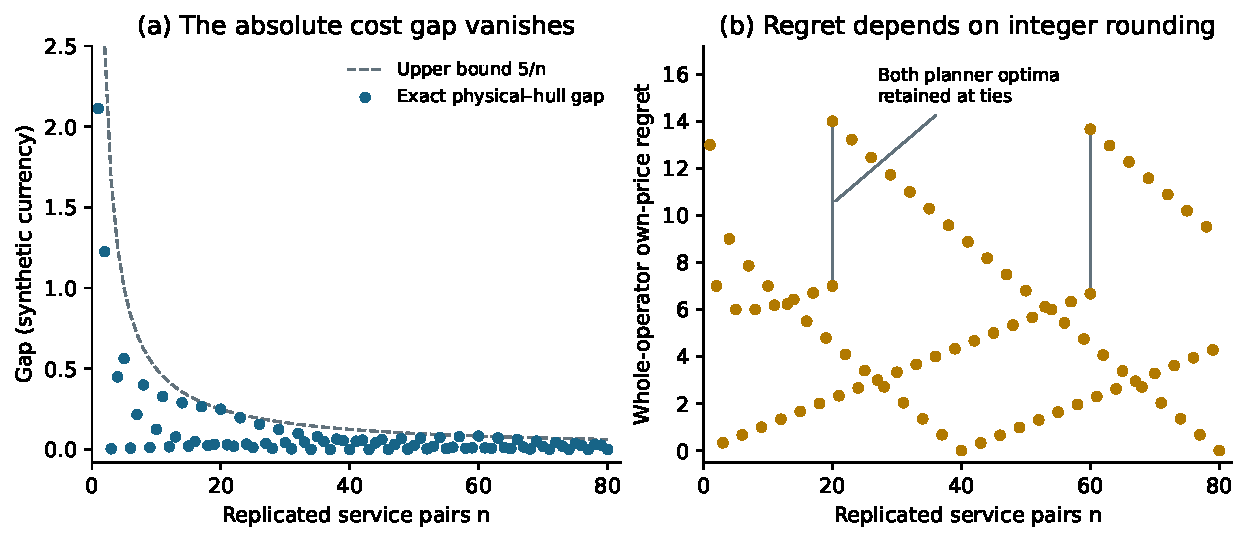
\includegraphics[width=.91\linewidth]{../figures/cyclic_replication.pdf}
\caption{Exact replication for $n=1,\ldots,80$, including both physical
optima at ties.  The planning gap follows the $5/n$ bound while
whole-operator own-price regret varies with integer rounding.  Values are
synthetic units, not observations from a bus system.}
\label{fig:exact-replication}
\end{figure}
